\subsubsection{Quản lý thành viên}

\begin{figure}[h]
    \centering
    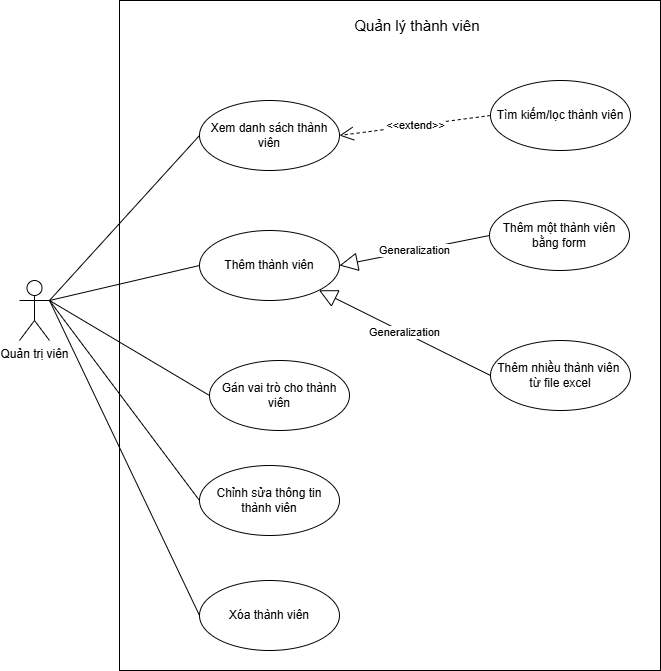
\includegraphics[width=1.0\linewidth]{Images/use-case-diagram/UC01_user_usecase.drawio.png}
    \vspace{0.3em}
    \caption{UC01 - Quản lý thành viên}
    \label{fig:uc01-usecase}
\end{figure}

% -----------------Bảng 1 use case tổng quát--------------------------
\begin{table}[H]
\centering
\renewcommand{\arraystretch}{1.3}
\begin{tabular}{|m{\dimexpr 0.25\textwidth-2\tabcolsep}|m{\dimexpr 0.75\textwidth-2\tabcolsep}|}
\hline
\textbf{Use-case Name}
& \textbf{UC01. Quản lý thành viên} \\ 
\hline

\textbf{Actors} 
& Quản trị viên \\ 
\hline

\textbf{Description} 
& Use case này cho phép quản trị viên thực hiện các thao tác quản lý thông tin thành viên trong hệ thống, bao gồm:
\begin{itemize}[label=--]
    \item Xem danh sách thành viên
    \item Tìm kiếm và lọc thành viên
    \item Thêm, sửa, xóa thông tin thành viên
    \item Gán vai trò (phân quyền) cho thành viên
\end{itemize} \\ 
\hline

\textbf{Trigger} 
& Quản trị viên truy cập chức năng Quản lý thành viên từ giao diện hệ thống. \\ 
\hline

\textbf{Pre-Conditions} 
& Quản trị viên đã đăng nhập vào hệ thống bằng tài khoản có quyền quản lý thành viên. \\ 
\hline

\textbf{Post-Conditions} 
& Thông tin thành viên được hiển thị và cập nhật chính xác theo các thao tác đã thực hiện. \\ 
\hline

\textbf{Normal Flow} 
&
\begin{enumerate}
    \item Quản trị viên truy cập module \textit{Quản lý thành viên}.
    \item Hệ thống hiển thị danh sách thành viên.
    \item Quản trị viên chọn một trong các thao tác:
    \begin{itemize}[label=--]
        \item Xem chi tiết thông tin thành viên
        \item Tìm kiếm hoặc lọc thành viên
        \item Thêm mới thành viên
        \item Chỉnh sửa thông tin thành viên
        \item Xóa thành viên
        \item Gán vai trò (phân quyền) cho thành viên
    \end{itemize}
    \item Hệ thống xử lý yêu cầu và cập nhật dữ liệu.
    \item Hệ thống hiển thị kết quả thao tác cho quản trị viên.
\end{enumerate}
\\ 
\hline

\textbf{Alternative Flow} 
& Ở bước 3:
\begin{itemize}[label=--]
    \item \textbf{3a.} Quản trị viên thực hiện tìm kiếm hoặc lọc thành viên, hệ thống hiển thị danh sách thành viên phù hợp với điều kiện tìm kiếm.
    \item \textbf{3b.} Quản trị viên chọn hủy thao tác thêm/sửa, hệ thống quay lại danh sách thành viên mà không thay đổi dữ liệu.
\end{itemize}
\\ 
\hline

\textbf{Exception} 
& Ở bước 1
\begin{itemize}[label=--]
    \item \textbf{1a.} Nếu quản trị viên không có quyền truy cập chức năng quản lý thành viên, hệ thống chặn truy cập và không hiển thị module này trên giao diện.
\end{itemize}
\\
& Ở bước 4:
\begin{itemize}[label=--]
    \item \textbf{4a.} Nếu dữ liệu nhập không hợp lệ, hệ thống hiển thị thông báo lỗi và yêu cầu quản trị viên nhập lại.
\end{itemize}
\\ 
\hline

\end{tabular}
\caption{Bảng mô tả Use Case UC01 – Quản lý thành viên}
\end{table}
% -----------------Bảng 2 use case thêm thành viên bằng form--------------------------
\begin{table}[H]
\centering
\renewcommand{\arraystretch}{1.3}
\begin{tabular}{|m{0.25\textwidth}|m{0.75\textwidth}|}
\hline
\textbf{Use-case Name} 
& \textbf{UC01.1. Thêm một thành viên từ Form} \\ 
\hline

\textbf{Actors} 
& Quản trị viên \\ 
\hline

\textbf{Description} 
& Quản trị viên thêm một thành viên mới vào hệ thống thông qua form nhập liệu. \\ 
\hline

\textbf{Trigger} 
& Quản trị viên bấm nút \textit{``Thêm thành viên mới''} trong trang quản lý người dùng. \\ 
\hline

\textbf{Pre-Conditions} 
&
\begin{itemize}[label=--]
    \item Quản trị viên đã đăng nhập vào hệ thống
    \item Quản trị viên có quyền tạo thành viên mới
\end{itemize}
\\ 
\hline

\textbf{Post-Conditions} 
&
\begin{itemize}[label=--]
    \item Thành viên mới được tạo và lưu vào cơ sở dữ liệu
    \item Mật khẩu mặc định được tạo tự động từ email hoặc mã số
    \item Thành viên được gán vào tổ chức (nếu có)
    \item Thành viên được gán vai trò (nếu có)
    \item Hệ thống gửi thông báo về mật khẩu mặc định cho thành viên
\end{itemize}
\\ 
\hline

\textbf{Normal Flow} 
&
\begin{enumerate}
    \item Quản trị viên bấm nút \textit{``Thêm thành viên mới''}.
    \item Hệ thống hiển thị form nhập thông tin thành viên với các trường:
    \begin{itemize}[label=--]
        \item \textbf{Bắt buộc}: Họ và tên đệm, Tên, Email, Mã số sinh viên/cán bộ
        \item \textbf{Tùy chọn}: Số điện thoại, Mật khẩu, Tổ chức, Loại thành viên, Trạng thái
    \end{itemize}
    \item Quản trị viên điền thông tin vào form.
    \item Quản trị viên chọn tổ chức (nếu có).
    \item Quản trị viên chọn vai trò và tổ chức áp dụng vai trò (nếu có).
    \item Quản trị viên bấm nút \textit{``Tạo mới''}.
    \item Hệ thống kiểm tra tính hợp lệ của dữ liệu.
    \item Hệ thống tự động tạo mật khẩu mặc định từ email hoặc mã số.
    \item Hệ thống lưu thông tin thành viên.
    \item Hệ thống hiển thị thông báo \textit{``Tạo thành viên thành công''}.
    \item Hệ thống chuyển hướng về trang danh sách thành viên.
\end{enumerate}
\\ 
\hline

\textbf{Alternative Flow} 
&
\begin{itemize}[label=--]
    \item \textbf{8.a.} Không cung cấp mật khẩu:
    \begin{itemize}[label=+]
        \item Hệ thống tạo mật khẩu từ phần trước ký tự \texttt{@} của email
        \item Nếu không có email, sử dụng mã số sinh viên/cán bộ
        \item Mật khẩu được mã hóa trước khi lưu
    \end{itemize}
\end{itemize}
\\ 
\hline

\textbf{Exception} 
&
\begin{itemize}[label=--]
    \item \textbf{7.a.} Email hoặc mã số đã tồn tại:
    \begin{itemize}[label=+]
        \item Hiển thị lỗi \textit{``Email hoặc mã số đã tồn tại trong hệ thống''}
        \item Quay lại bước 3
    \end{itemize}
    \item \textbf{7.b.} Thiếu trường bắt buộc:
    \begin{itemize}[label=+]
        \item Hiển thị lỗi \textit{``Vui lòng điền đầy đủ thông tin bắt buộc''}
        \item Quay lại bước 3
    \end{itemize}
\end{itemize}
\\ 
\hline

\end{tabular}
\caption{Bảng mô tả Use Case UC01.1 - Thêm một thành viên từ Form}
\end{table}

% -----------------Bảng 3 use case thêm thành viên từ file excel--------------------------
\begin{table}[H]
\centering
\renewcommand{\arraystretch}{1.3}
\begin{tabular}{|m{0.25\textwidth}|m{0.75\textwidth}|}
\hline
\textbf{Use-case Name} 
& \textbf{UC01.2. Thêm nhiều thành viên từ file Excel} \\ 
\hline

\textbf{Actors} 
& Quản trị viên \\ 
\hline

\textbf{Description} 
& Quản trị viên thêm hàng loạt thành viên từ file Excel theo template chuẩn gồm 18 cột dữ liệu. \\ 
\hline

\textbf{Trigger} 
& Quản trị viên cần thêm nhiều thành viên cùng lúc (ví dụ: đầu năm học, import danh sách sinh viên mới). \\ 
\hline

\textbf{Pre-Conditions} 
&
\begin{itemize}[label=--]
    \item Quản trị viên đã đăng nhập vào hệ thống
    \item Quản trị viên có quyền import thành viên
    \item File Excel đã được chuẩn bị theo template chuẩn
\end{itemize}
\\ 
\hline

\textbf{Post-Conditions} 
&
\begin{itemize}[label=--]
    \item Danh sách thành viên được import thành công
    \item Các tổ chức được tự động tạo nếu chưa tồn tại
    \item Mật khẩu mặc định được tạo cho mỗi thành viên
    \item Hệ thống ghi log chi tiết quá trình import
    \item Báo cáo kết quả import được tạo
\end{itemize}
\\ 
\hline

\textbf{Normal Flow} 
&
\begin{enumerate}
    \item Quản trị viên bấm nút \textit{``Thêm từ File''}.
    \item Hệ thống hiển thị hướng dẫn và nút tải file mẫu.
    \item Quản trị viên tải template Excel (18 cột).
    \item Quản trị viên điền dữ liệu vào template.
    \item Quản trị viên upload file Excel.
    \item Hệ thống nhận file và tạo session import.
    \item Hệ thống parse file và trả về \texttt{sessionId}.
    \item Quản trị viên bấm \textit{``Validate dữ liệu''}.
    \item Hệ thống thực hiện validation và hiển thị kết quả.
    \item Quản trị viên bấm \textit{``Thực hiện import''}.
    \item Hệ thống import dữ liệu theo batch.
    \item Hệ thống hiển thị tiến trình import real-time.
    \item Hệ thống hiển thị báo cáo kết quả import.
\end{enumerate}
\\ 
\hline

\textbf{Alternative Flow} 
&
\begin{itemize}[label=--]
    \item \textbf{13.a.} Tự động tạo tổ chức:
    \begin{itemize}[label=+]
        \item Phát hiện mã khoa/lớp chưa tồn tại
        \item Tạo tổ chức mới
        \item Gán thành viên vào tổ chức vừa tạo
    \end{itemize}
\end{itemize}
\\ 
\hline

\textbf{Exception} 
&
\begin{itemize}[label=--]
    \item \textbf{6.a.} File không đúng định dạng (.xlsx)
    \item \textbf{6.b.} File quá lớn (>$10$MB)
    \item \textbf{6.c.} File không đúng template
    \item \textbf{9.a.} 100\% bản ghi có lỗi nghiêm trọng
\end{itemize}
\\ 
\hline

\end{tabular}
\caption{Bảng mô tả Use Case UC01.2 - Thêm nhiều thành viên từ file Excel}
\end{table}

% -----------------Bảng 4 use case gán vai trò cho thành viên--------------------------
\renewcommand{\arraystretch}{1.3}
\begin{longtable}{|m{0.25\textwidth}|m{0.75\textwidth}|}
 \hline

\textbf{Use-case Name} & \textbf{UC01.3. Gán vai trò cho thành viên} \\ \hline
\endfirsthead

\hline
\textbf{Use-case Name (tiếp)} & \textbf{UC01.3. Gán vai trò cho thành viên} \\ \hline
\endhead

% ===== Nội dung bảng =====
\textbf{Actors} 
& Quản trị viên \\ 
\hline

\textbf{Description} 
& Quản trị viên gán một hoặc nhiều vai trò cho thành viên. Mỗi vai trò có thể được gán trong phạm vi tổ chức cụ thể hoặc trên toàn hệ thống. \\ 
\hline

\textbf{Trigger} 
& Quản trị viên cần phân quyền cho thành viên để họ thực hiện các chức năng trong hệ thống. \\ 
\hline

\textbf{Pre-Conditions} 
&
\begin{itemize}[label=--]
    \item Quản trị viên đã đăng nhập vào hệ thống
    \item Quản trị viên có quyền gán vai trò
    \item Thành viên đã tồn tại trong hệ thống
    \item Hệ thống đã có các vai trò được định nghĩa
\end{itemize}
\\ 
\hline

\textbf{Post-Conditions} 
&
\begin{itemize}[label=--]
    \item Thành viên được gán vai trò mới
    \item Quyền hạn của thành viên được cập nhật theo vai trò
    \item Lịch sử gán vai trò được ghi log
    \item Thành viên có thể thực hiện các chức năng theo quyền mới
\end{itemize}
\\ 
\hline

\textbf{Normal Flow} 
&
\begin{enumerate}
    \item Quản trị viên truy cập trang chi tiết thành viên.
    \item Hệ thống hiển thị thông tin thành viên và danh sách vai trò hiện tại.
    \item Quản trị viên bấm nút \textit{``Gán vai trò''}.
    \item Hệ thống hiển thị form gán vai trò với:
    \begin{itemize}[label=--]
        \item Dropdown chọn vai trò (Super Admin, Quản lý đóng phí, \ldots)
        \item Dropdown chọn tổ chức áp dụng (tủy chọn)
    \end{itemize}
    \item Quản trị viên chọn vai trò từ danh sách.
    \item Quản trị viên chọn tổ chức áp dụng vai trò (nếu vai trò yêu cầu phạm vi).
    \item Quản trị viên bấm nút \textit{``Lưu''}.
    \item Hệ thống kiểm tra vai trò--tổ chức không bị trùng lặp.
    \item Hệ thống lưu thông tin vai trò mới cho thành viên.
    \item Hệ thống cập nhật quyền hạn của thành viên.
    \item Hệ thống hiển thị thông báo \textit{``Gán vai trò thành công''}.
    \item Danh sách vai trò của thành viên được cập nhật.
\end{enumerate}
\\ 
\hline

\textbf{Alternative Flow} 
&
\begin{itemize}[label=--]
    \item \textbf{6.a.} Không chọn tổ chức (vai trò toàn hệ thống):
    \begin{itemize}[label=+]
        \item Quản trị viên bỏ trống trường tổ chức
        \item Vai trò được gán ở phạm vi toàn hệ thống
        \item Thành viên có quyền hạn trong tất cả tổ chức
    \end{itemize}

    \item \textbf{7.a.} Gán nhiều vai trò cùng lúc:
    \begin{itemize}[label=+]
        \item Sau khi lưu vai trò đầu tiên, bấm \textit{``Thêm vai trò khác''}
        \item Lặp lại bước 5--7 cho mỗi vai trò
        \item Hệ thống lưu tất cả các vai trò
    \end{itemize}

    \item \textbf{7.b.} Xóa vai trò hiện tại:
    \begin{itemize}[label=+]
        \item Bấm nút \textit{``Xóa''} tại vai trò cần xóa
        \item Hệ thống hiển thị xác nhận xóa
        \item Quản trị viên xác nhận
        \item Hệ thống xóa vai trò và cập nhật quyền hạn
    \end{itemize}

    \item \textbf{7.c.} Cập nhật toàn bộ vai trò:
    \begin{itemize}[label=+]
        \item Truy cập chế độ \textit{``Chỉnh sửa vai trò''}
        \item Thêm hoặc xóa các vai trò theo nhu cầu
        \item Bấm \textit{``Lưu tất cả''}
        \item Hệ thống xóa toàn bộ vai trò cũ
        \item Hệ thống gán lại các vai trò mới
    \end{itemize}
\end{itemize}
\\ 
\hline

\textbf{Exception} 
&
\begin{itemize}[label=--]
    \item \textbf{8.a.} Vai trò--tổ chức đã tồn tại:
    \begin{itemize}[label=+]
        \item Phát hiện vai trò đã được gán cho thành viên trong tổ chức này
        \item Hiển thị lỗi \textit{``Thành viên đã có vai trò này trong tổ chức đã chọn''}
        \item Quay lại bước 5
    \end{itemize}

    \item \textbf{8.b.} Vai trò yêu cầu tổ chức nhưng không được chọn:
    \begin{itemize}[label=+]
        \item Hiển thị lỗi \textit{``Vai trò này yêu cầu chọn tổ chức áp dụng''}
        \item Quay lại bước 6
    \end{itemize}

    \item \textbf{8.c.} Không đủ quyền gán vai trò:
    \begin{itemize}[label=+]
        \item Không có quyền gán vai trò cấp cao (ví dụ: Admin)
        \item Hiển thị lỗi \textit{``Bạn không có quyền gán vai trò này''}
        \item Quay lại bước 5
    \end{itemize}
\end{itemize}
\\ \hline
\caption{Bảng mô tả Use Case UC01.3 - Gán vai trò cho thành viên}
\end{longtable}
